\documentclass{beamer}
\usetheme{Boadilla}

\usepackage[utf8]{inputenc}
\usepackage{amsmath}
\usepackage{booktabs}

\newcommand{\argmax}[1]{\underset{#1}{\operatorname{argmax}}\;}

\title{Advanced Numerical Mathematics}
\subtitle{Finite difference method for solving boundary value problems}
\author{Marcel Gohsen}
\institute{Bauhaus-Universit\"at Weimar}

\begin{document}
	\frame{\titlepage}
	
	\begin{frame}{The problem}
		\textbf{Differential equation}: \\
		$$y''(x) + y(x) = 3 \sin x$$ 
		\textbf{Boundary conditions}: \\
		\begin{align*}
			y(0) + y'(0) &= 0\\
			y(\frac{\pi}{2}) + y'(\frac{\pi}{2}) &= 0
		\end{align*}
		
		Find solutions $x$ to the differential equation which satisfy the boundary conditions.
	\end{frame}
	
	\begin{frame}{Finite difference method}
		Solve differential equations with the help of finite differences to approximate derivatives. \\~\\
		
		
		\textbf{Introduce discretization on a grid}\\
		Given: boundary values $a$, $b$, the number of steps $N$  
		\begin{align*}
			h &= \frac{b - a}{N - 1}\\
			x_i &= a + (i - 1)h\quad\text{with}\ i\in[1, N]
		\end{align*}
		
		
		
	\end{frame}
	
	\begin{frame}{Finite difference method}
		\textbf{Discretization of problem}
		\begin{align*}
			a &= 0,\ b= \frac{\pi}{2},\ N = 10\\
			h &= \frac{\frac{\pi}{2} - 0}{10 - 1} = \frac{\pi}{18}\\~\\
			x &= \{0 \cdot \frac{\pi}{18}, 1 \cdot \frac{\pi}{18},\ldots, 9 \cdot \frac{\pi}{18}\}
		\end{align*}
		
	\end{frame}
	
	\begin{frame}{Finite difference operators}
		\textbf{First-order}
		\begin{align*}
			\text{Forward:}\ y'(x_{i}) &\approx \frac{y(x_{i+1}) - y(x_{i})}{h}\\
			\text{Backward:}\ y'(x_{i}) &\approx \frac{y(x_{i}) - y(x_{i-1})}{h}\\
			\text{Central:}\ y'(x_{i}) &\approx \frac{y(x_{i+1}) - y(x_{i-1})}{2h}\\
		\end{align*}
		\textbf{Second-order}
		$$y''(x_i) \approx \frac{y(x_{i-1}) - 2y(x_i) + y(x_{i+1})}{h^2}$$
	\end{frame}
	
	\begin{frame}{Finite difference operators}
		Approximate derivatives in the differential equation with finite difference operators:
		\begin{align*}
			y''(x_i) + y(x_i) &= 3 \sin x_i\\
			\frac{y(x_{i-1}) - 2y(x_i) + y(x_{i+1})}{h^2} + y(x_i) &= 3 \sin x_i\\
			\frac{y(x_{i-1}) + (h^2 - 2)y(x_i) + y(x_{i+1})}{h^2} &= 3 \sin x_i\\
			y(x_{i-1}) + (h^2 - 2)y(x_i) + y(x_{i+1}) &= 3 h^2\sin x_i
		\end{align*}		 
	\end{frame}
	
	\begin{frame}{Finite difference method}
		Build linear equation system for \textit{interior points} of discretization 
		\begin{align*}
			\text{for}\ i=2&:\ y(x_1) + (h^2 - 2)y(x_2) + y(x_3) = 3h^2\sin x_2\\
			\text{for}\ i=3&:\ y(x_2) + (h^2 - 2)y(x_3) + y(x_4) = 3h^2\sin x_3\\
			\text{for}\ i=4&:\ y(x_3) + (h^2 - 2)y(x_4) + y(x_5) = 3h^2\sin x_4\\
			&\qquad\vdots\\
			\text{for}\ i=9&:\ y(x_8) + (h^2 - 2)y(x_9) + y(x_{10}) = 3h^2\sin x_9
		\end{align*}
	\end{frame}
	
	\begin{frame}{Boundary conditions}
		\begin{align*}
			y(x_1) + y'(x_1) &= 0\\
			y(x_{10}) + y'(x_{10}) &= 0
		\end{align*}
		
		Approximate derivatives in boundary conditions with finite differences. 
		\begin{align*}
			y(x_1) + \frac{y(x_{2}) - y(x_{1})}{h} &= 0\\
			(h-1)y(x_1)+ y(x_{2}) &= 0\\~\\
			y(x_{10}) + \frac{y(x_{10}) - y(x_{9})}{h} &= 0\\
			-y(x_9) + (h+1) y(x_{10}) &= 0\\~\\
		\end{align*}
	\end{frame}
	
	\begin{frame}{Linear equation system}
		The final linear equation system: 
		\begin{equation*}
		\Tiny
			\begin{pmatrix}
				h-1 & 1 & 0 & 0 & 0 & 0 & 0 & 0 & 0 & 0\\
				1 & h^2 - 2 & 1 & 0 & 0 & 0 & 0 & 0 & 0 & 0\\
				0 & 1 & h^2 - 2 & 1 & 0 & 0 & 0 & 0 & 0 & 0\\
				0 & 0 & 1 & h^2 - 2 & 1 & 0 & 0 & 0 & 0 & 0\\
				0 & 0 & 0 & 1 & h^2 - 2 & 1 & 0 & 0 & 0 & 0\\
				0 & 0 & 0 & 0 & 1 & h^2 - 2 & 1 & 0 & 0 & 0\\
				0 & 0 & 0 & 0 & 0 & 1 & h^2 - 2 & 1 & 0 & 0\\
				0 & 0 & 0 & 0 & 0 & 0 & 1 & h^2 - 2 & 1 & 0\\
				0 & 0 & 0 & 0 & 0 & 0 & 0 & 1 & h^2 - 2 & 1\\
				0 & 0 & 0 & 0 & 0 & 0 & 0 & 0 & -1 & h+1\\
			\end{pmatrix}
			\begin{pmatrix}
				y(x_0)\\
				y(x_1)\\
				y(x_2)\\
				y(x_3)\\
				y(x_4)\\
				y(x_5)\\
				y(x_6)\\
				y(x_7)\\
				y(x_8)\\
				y(x_9)\\
				y(x_{10})
			\end{pmatrix} = 
			\begin{pmatrix}
				0\\
				3h^2\sin x_2\\
				3h^2\sin x_3\\
				3h^2\sin x_4\\
				3h^2\sin x_5\\
				3h^2\sin x_6\\
				3h^2\sin x_7\\
				3h^2\sin x_8\\
				3h^2\sin x_9\\
				0
			\end{pmatrix}
		\end{equation*}
	\end{frame}
	
	\begin{frame}{Solvers}
		Solving of the linear equation system is implemented with the following methods: \\~\\
		Direct methods:\\
		\begin{itemize}
			\item Classical Gaussian Elimination\\
			\item Gaussian Elimination with pivot selection
		\end{itemize}
		
		Iterative methods:
		\begin{itemize}
			\item Jacobi method
			\item Successive over-relaxation (SOR) 
		\end{itemize}
	\end{frame}
	
	\begin{frame}{Classical Gaussian Elimination}
		Let us consider a linear equation system $Ax = b$ with
		\begin{equation*}
			A = 
			\begin{pmatrix}
				a_{1,1}	& a_{1,2} & \cdots & a_{1,m}\\
				a_{2,1} & a_{2,2} & \cdots & a_{2,m}\\
				\vdots & & &\\
				a_{m,1} & a_{m, 2} & \cdots & a_{m,m}
			\end{pmatrix} \quad b = \begin{pmatrix}
				b_1\\
				b_2\\
				\vdots\\
				b_m
			\end{pmatrix}
		\end{equation*}
		We compute factors in the $k$-th step $\mu_{i,k}$ with $k=1,...,m-1$ and  $i=k+1,...,m$. 
		\begin{equation*}
			\mu_{i,k} = \frac{a_{i,k}^{(k-1)}}{a_{k,k}^{(k-1)}}
		\end{equation*}
		Multiply the $k$-th row  with factor and subtract from $k+1,...,m$ row to obtain \textit{row echelon form} (Stufenform). Back-substitution yields result $x$. 
	\end{frame}

	\begin{frame}{Gaussian Elimination with pivot selection}
	Search for the maximum pivot in $k$-th step $a_{i,j}^{(k-1)}$ with $k=1,...,m-1$ $i=k,...,m$ and $j=k,...,m$. 
		\begin{equation*}
			(i_{max},j_{max}) = \argmax{i,j} a_{i,j}^{(k-1)}
		\end{equation*}
		Swap $k$-th row with $i_{max}$ row and compute factors.
		\begin{equation*}
			\mu_{i,j_{max}} = \frac{a_{i,j_{max}}^{(k-1)}}{a_{i_{max},j_{max}}^{(k-1)}}
		\end{equation*}
		Multiply the $k$-th row  with factor and subtract from $k+1,...,m$ row to obtain \textit{row echelon form} (Stufenform). Back-substitution yields result $x$. 
	\end{frame} 
	
	\begin{frame}{Jacobi method}
		$$(L + D + U)x = b$$
		$$x = -D^{-1}(L+U)x + D^{-1}b$$
		
		Iteration:
		\begin{align*}
			C &= -D^{-1}(L+U)\\
			d &= D^{-1}b\\
			x^{(k+1)} &= Cx^{(k)} + d
		\end{align*}
		with an initial guess $x_0$.\\
		Convergence:
		$$\sum_{j=1, j\neq i}^{m} |a_{i,j}| < |a_{j,j}|$$ 
		$\Rightarrow A$ must be \textit{diagonally dominant}!
	\end{frame}
	
	\begin{frame}{Successive over-relaxation (SOR)}
		$$Lx + Dx + Ux = b$$
		$$x = x + D^{-1}(b-Lx-Rx-Dx)$$
		Introducing a relaxation factor $\omega$ with $0<\omega<2 $ \\
		Iteration:
		\begin{align*}
			x^{(k+1)} &= x^{(k)} + \omega D^{-1}(b - Lx^{(k+1)} - Rx^{(k)} - D x^{(k)})
		\end{align*}
	\end{frame}
	
	\begin{frame}{Evaluation}
		Exact solutions of the problem described by: 
		\begin{equation*}
			\hat{y}(x)= \frac{3}{8}\left(\left(\pi+2\right)\cos x - \left(\pi - 2\right)\sin x\right) - \frac{3}{2}x\cos x
		\end{equation*}
		Error calculations:
		\begin{align*}
			\text{Absolute error}&:\ ||\hat{y} - y||\\
			\text{Relative error}&:\ \frac{||\hat{y} - y||}{||\hat{y}||}
		\end{align*}
	\end{frame}
	
	\begin{frame}{Evaluation}
		\begin{table}
			\begin{tabular}{c| r r r r r r}
				\toprule
				$n$ & \multicolumn{2}{c}{Gauss} & \multicolumn{2}{c}{Gauss with PS} & \multicolumn{2}{c}{SOR}\\
				 & Abs & Rel & Abs & Rel & Abs & Rel \\
				\midrule
				10 & 0.3962 & 0.1330 & 0.3962 & 0.1330 & 0.4102 & 0.1377 \\
				50 & 0.1785 & 0.0285 & 0.1785 & 0.0285 & 2.6691 & 0.4268\\
				100 & 0.1263 & 0.0144 & 0.1263 & 0.0144 & 4.7574 & 0.5422\\
				\bottomrule			
			\end{tabular}
		\end{table}
		
		Jacobi method: The equation system obtained by finite difference method is not diagonally dominant and thus achieves no convergence towards the solution. 
	\end{frame}
	
	\begin{frame}{Evaluation}
		\begin{figure}
			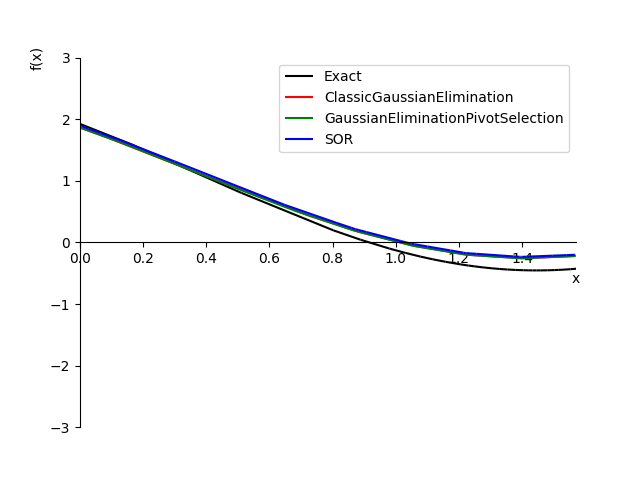
\includegraphics[width=.8\textwidth]{evaluation_tex.png}
			\caption{Plot of the solution with $n=10$}
		\end{figure}
	\end{frame}
\end{document}